\chapter{DATA PREPROCESSING AND FEATURE ENGINEERING}

\section{Data Cleaning}

The validation stage in \texttt{src/data\_loader.py} produces a JSON record of
every check, and the report quotes that record rather than the repository
description. The findings were as follows.

\textbf{Missing values.} None, in any column. No imputation was required, and no
imputation step exists in the pipeline. This is worth stating explicitly because
it removes a common source of leakage: there is no imputed statistic that could
be computed on the full dataset before the split.

\textbf{Non-finite and invalid values.} No infinite values, no negative values
and no constant columns. All 16 features are strictly positive, which is
consistent with them being geometric measurements.

\textbf{Target labels.} The class column contains exactly the seven expected
labels, in upper case, with no trailing whitespace and no unexpected category.
No mapping was applied; the strings are used directly as class identifiers, and
scikit-learn stores them as the estimator's \texttt{classes\_} attribute in
alphabetical order (BARBUNYA, BOMBAY, CALI, DERMASON, HOROZ, SEKER, SIRA). All
tables in this report are re-ordered to the variety order used in the source
publication so that they can be read against \cite{koklu2020}.

\textbf{Duplicate records.} \DuplicateRows{} rows are exact repeats of an earlier
row across all 17 columns. They were retained, for three reasons. First, the
features are derived from integer pixel counts and from ratios of those counts,
so two distinct beans of almost identical size and shape can produce identical
measurements; a duplicate is evidence of discretisation, not of a copying error.
Second, the duplicates are spread across varieties and amount to 0.5\% of the
data, so removing them would change the class balance slightly and the conclusions
not at all. Third, deleting them would be a decision made after seeing the test
set composition, which is exactly the kind of judgement the protocol in
Section~4.4 is designed to prevent. The duplicate count is reported as a
limitation in Section~7.2.

\textbf{Outliers.} Retained, as justified in Section~3.4.8. No observation was
winsorised, clipped or removed, and no log transformation was applied. The two
model families that would be affected by heavy tails, the linear and
kernel models, are protected by standardisation; the tree ensembles are
invariant to monotone transformations of individual features.

\section{Encoding and Feature Scaling}

\textbf{Target encoding.} The seven varieties are nominal with no order, so no
ordinal encoding is appropriate. The string labels are passed directly to
scikit-learn, which encodes them internally and decodes predictions back to
strings. This keeps every artefact, including the confusion matrices and the saved
model, in the original vocabulary and avoids an index-to-name mapping that could
silently drift between scripts.

\textbf{Feature scaling.} Standardisation is applied as
\begin{equation}
  z_{j} = \frac{x_{j} - \hat{\mu}_{j}}{\hat{\sigma}_{j}},
  \label{eq:zscore}
\end{equation}
where $\hat{\mu}_{j}$ and $\hat{\sigma}_{j}$ are the mean and standard deviation
of feature $j$ estimated on the training data only. The scaler is not applied to
the tree ensembles. A decision tree splits on a threshold $x_j \le t$; replacing
$x_j$ by an affine function of $x_j$ changes the threshold but not the partition,
so standardisation cannot change a forest's predictions and would only add work.
For logistic regression, kNN and the SVM the situation is the opposite:
standardisation is not cosmetic but constitutive.

The effect is easy to quantify. In raw units, \texttt{Area} has a standard
deviation of 29,324 and \texttt{ShapeFactor2} a standard deviation of 0.0006. In a
Euclidean distance, the contribution of a one-standard-deviation change in
\texttt{Area} exceeds that of \texttt{ShapeFactor2} by a factor of roughly
$5\times10^{7}$. A kNN classifier fitted on raw values would therefore be a
one-dimensional classifier on \texttt{Area}, and an RBF kernel would compute
similarities that are effectively $\exp(-\gamma\,\|\Delta\text{Area}\|^2)$.

\textbf{Leakage control.} The scaler is the first step of a scikit-learn
\texttt{Pipeline}, and the pipeline is what the search object clones and fits on
each training fold. The test partition is never passed to \texttt{fit}. The
practical consequence is that each cross-validation fold estimates
$\hat{\mu}$ and $\hat{\sigma}$ from its own training portion, so the reported
cross-validation scores are honest estimates of out-of-sample performance rather
than mildly optimistic ones. Listing~\ref{lst:pipeline} shows the construction.

\begin{lstlisting}[style=pycode, caption={Pipeline construction: the scaler is
fitted inside cross-validation, never before it.}, label={lst:pipeline}]
def build_pipeline(estimator, scale: bool) -> Pipeline:
    steps = [("scaler", StandardScaler())] if scale else []
    steps.append(("model", estimator))
    return Pipeline(steps)
\end{lstlisting}

\section{Feature Selection and Feature Engineering}

No feature was added. The 16 descriptors are the published feature set, and
engineering new ratios from them would duplicate information that
\texttt{ShapeFactor1} to \texttt{ShapeFactor4} already encode. The relevant
question raised by the correlation analysis is the opposite one: can some columns
be removed?

The redundant cluster is the set of size features that measure the same
quantity: \texttt{Perimeter}, \texttt{MajorAxisLength}, \texttt{MinorAxisLength},
\texttt{ConvexArea} and \texttt{EquivDiameter}. All five correlate with
\texttt{Area} at between 0.93 and 0.99. A controlled ablation was run: a Random
Forest with the hyperparameters selected for the full feature set was
cross-validated twice, once on all 16 columns and once on the 11 columns that
remain after dropping that cluster. Table~\ref{tab:ablation} reports the result.

\begin{table}[htbp]
\centering
\small
\caption{Effect of dropping the five redundant size features (Random Forest, identical hyperparameters)}
\label{tab:ablation}
\begin{tabular}{lcrr}
\toprule
Feature set & Features & CV macro F1 & Std. dev. \\
\midrule
all 16 features & 16 & 0.9362 & 0.0031 \\
11 features reduced & 11 & 0.9372 & 0.0029 \\
\bottomrule
\end{tabular}
\end{table}


Removing five of the 16 features changes the cross-validated macro F1 from
\AblationFull{} to \AblationReduced{}, an improvement of about 0.001 that is
smaller than the fold-to-fold standard deviation of either configuration. The
difference is not evidence that the reduced set is better; it is evidence that the
two sets carry the same information. Given that, the full set was kept, because
the redundant columns cost almost nothing at prediction time and the published
literature reports results on all 16, which keeps the comparison in Chapter~6
like-for-like.

The honest statement is that feature selection was tested and did not improve
generalisation. That is a more useful outcome than a claim that 16 features are
necessary.

\section{Training, Validation and Test Split}

The cleaned dataset was divided once, by stratified random sampling, into 80\%
training and 20\% test with \texttt{random\_state = 42}. Stratification keeps the
class proportions of the full dataset in both partitions, which matters for
Bombay: a plain random split could leave the test set with fewer than 90 Bombay
beans and make its per-class F1 unstable. Table~\ref{tab:split} shows the
resulting counts and Figure~\ref{fig:splitbar} the proportions.

\begin{table}[htbp]
\centering
\small
\caption{Stratified 80/20 partition: class counts are preserved in both subsets}
\label{tab:split}
\begin{tabular}{lrrrr}
\toprule
Variety & Full dataset & Share (\%) & Training & Test \\
\midrule
Seker & 2,027 & 14.9 & 1,621 & 406 \\
Barbunya & 1,322 & 9.7 & 1,057 & 265 \\
Bombay & 522 & 3.8 & 418 & 104 \\
Cali & 1,630 & 12.0 & 1,304 & 326 \\
Dermason & 3,546 & 26.1 & 2,837 & 709 \\
Horoz & 1,928 & 14.2 & 1,542 & 386 \\
Sira & 2,636 & 19.4 & 2,109 & 527 \\
\bottomrule
\end{tabular}
\end{table}


\begin{figure}[htbp]
\centering
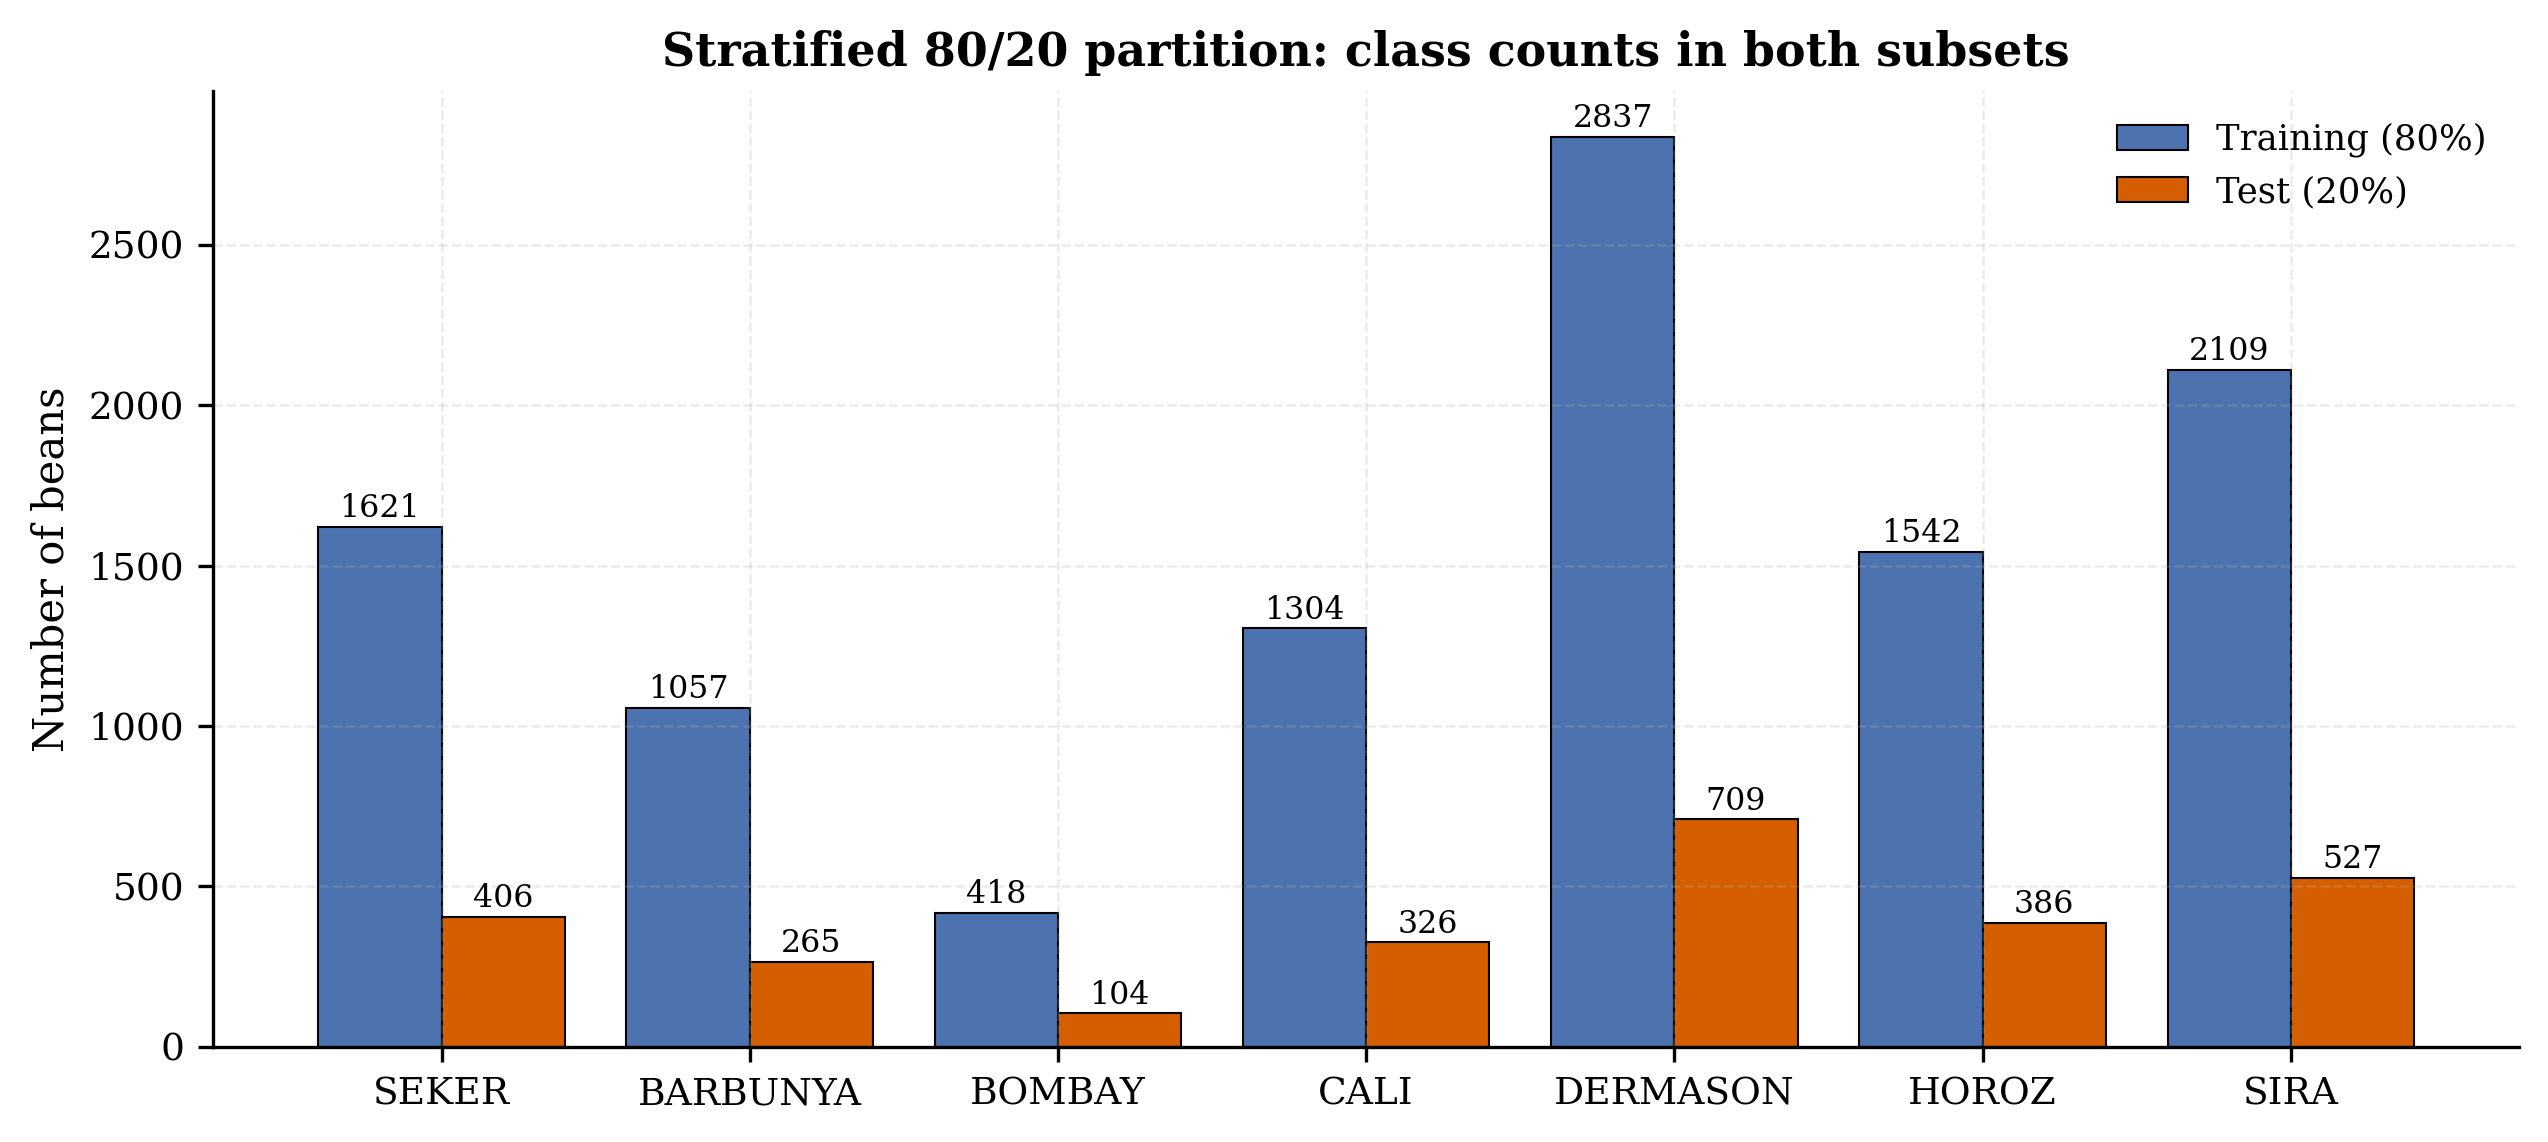
\includegraphics[width=0.80\textwidth]{fig_4_1_split.png}
\caption{Stratified partition of the dataset. The class proportions are preserved
to within 0.1 percentage points in both subsets.}
\label{fig:splitbar}
\end{figure}

The training partition supplies both model fitting and model selection: the
hyperparameter search uses stratified five-fold cross-validation inside the
\TrainRows{} training beans, so each candidate configuration is scored on five
disjoint validation folds of roughly 2,178 beans. The test partition of
\TestRows{} beans is evaluated once, in Chapter~6, after the model has been
chosen. No test observation influences the choice of algorithm, the search space
or any hyperparameter value.

Four leakage controls were enforced and are checked by the test suite:

\begin{enumerate}[label=(\alph*)]
  \item the split is written to \texttt{data/processed/} and every later stage
        reads those files, so the partition cannot drift between experiments;
  \item the scaler is fitted inside the pipeline, on training folds only;
  \item no oversampling, undersampling or class weighting is applied before the
        split; class weighting is evaluated as a controlled experiment inside
        cross-validation (Table~\ref{tab:class_weight});
  \item the feature ablation in Section~4.3 uses cross-validation on the training
        partition only, so the comparison cannot be biased by test data.
\end{enumerate}

The class-imbalance experiment deserves a note. The literature reviewed in
Chapter~2 suggests resampling the minority classes \cite{lee2024}. Rather than
adopt that recommendation, the effect of balanced class weights was measured on
the training partition with the same folds used for model selection. The result,
in Table~\ref{tab:class_weight}, is that balanced weights lower the
cross-validated macro F1 of the selected model from \CWNone{} to \CWBalanced{}.
The original class distribution was therefore kept throughout. The reason is
visible in Figure~\ref{fig:class_distribution}: with 522 Bombay beans and a
feature that separates them almost perfectly, the minority class is not being
suppressed by the majority; reweighting only distorts the decision boundary
elsewhere.

\begin{table}[htbp]
\centering
\small
\caption{Effect of balanced class weights on the selected model}
\label{tab:class_weight}
\begin{tabular}{llrr}
\toprule
Model & class\_weight & CV macro F1 & Std. dev. \\
\midrule
RBF-SVM & none & 0.9420 & 0.0052 \\
RBF-SVM & balanced & 0.9407 & 0.0052 \\
\bottomrule
\end{tabular}
\end{table}

